\documentclass[a4paper,10pt]{article}
\usepackage[utf8]{inputenc}
%\usepackage[francais]{babel}
\usepackage[T1]{fontenc}
\usepackage{graphicx}
\usepackage{eurosym}
\usepackage{verbatim}
\usepackage{amsmath, amsthm}
\usepackage{latexsym}
\usepackage{amssymb}
\usepackage{tabularx}
\usepackage{setspace}
\usepackage{listings}
\usepackage{geometry}
\usepackage{fancyhdr}
%\usepackage{enumitem}
\usepackage{colortbl}
%\usepackage[dvipsnames]{xcolor}
\usepackage{booktabs}
%\usepackage{moreverb}

%\usepackage{cite}
\DeclareMathAlphabet{\mathonebb}{U}{bbold}{m}{n}
\newcommand{\one}{\ensuremath{\mathonebb{1}}}

\usepackage{color}
%\usepackage{multirow}
%\usepackage{float}
\definecolor{gris25}{gray}{0.75}
\usepackage{colortbl}
\usepackage{fancyhdr}
\usepackage{amsmath,amsfonts,amssymb}
%\usepackage{titlesec}
%\usepackage{supertabular}
\usepackage{longtable}

\usepackage{caption}
\usepackage{subcaption}


\usepackage{listings}
\definecolor{dkgreen}{rgb}{0,0.4,0}
\definecolor{gray}{rgb}{0.5,0.5,0.5}
\definecolor{mauve}{rgb}{0.58,0,0.82}


\usepackage[numbers]{natbib}

\newcommand\Mycite[1]{%
  \citeauthor{#1}~(\citeyear{#1})~\cite{#1}}


\usepackage{multicol}


%\usepackage{algorithm2e}

% marges,etc.
%\usepackage{a4wide}
\hoffset -1cm
\voffset -2cm
\textheight 25cm
\headheight 1cm
\headsep 1cm
\topmargin 0cm
\textwidth 16cm

%to change temporaly a margin
\def\changemargin#1#2{\list{}{\rightmargin#2\leftmargin#1}\item[]}
\let\endchangemargin=\endlist 


%pour les couleurs
\usepackage{color}
\definecolor{mycolor}{rgb}{0.06,0.32,0.39}

%liens dans le corps du texte
\usepackage{hyperref}
\hypersetup{
    colorlinks=true,
    linkcolor=blue,
    citecolor=dkgreen,
    filecolor=blue,
    urlcolor=blue,
}

\urlstyle{same}

\definecolor{dkyellow}{cmyk}{0, 0, 0.2, 0}
\lstset{
  language=Python,                % the language of the code
  basicstyle= \footnotesize,      % the size of the fonts that are used for the code
  numbers=left,                   % where to put the line-numbers
  numberstyle=\tiny\color{gray},  % the style that is used for the line-numbers
  stepnumber=2,                   % the step between two line-numbers. If it's 1, each line
                                  % will be numbered
  showspaces=false,               % show spaces adding particular underscores
  showtabs=false,                 % show tabs within strings adding particular underscores
  frame=single,                   % adds a frame around the code
  rulecolor=\color{black},        % if not set, the frame-color may be changed on line-breaks within not-black text (e.g. commens (green here))
  tabsize=2,                      % sets default tabsize to 2 spaces
  captionpos=b,                   % sets the caption-position to bottom
  breaklines=true,                % sets automatic line breaking
  breakatwhitespace=false,        % sets if automatic breaks should only happen at whitespace
  keywordstyle=\color{blue},      % keyword style
  commentstyle=\color{dkgreen},   % comment style
  stringstyle=\color{mauve},       % string literal style
  backgroundcolor=\color{white},      % choose the background color. You must add \usepackage{color}
}

\usepackage{array}
\newcolumntype{L}[1]{>{\raggedright\let\newline\\\arraybackslash\hspace{0pt}}m{#1}}
\newcolumntype{C}[1]{>{\centering\let\newline\\\arraybackslash\hspace{0pt}}m{#1}}
\newcolumntype{R}[1]{>{\raggedleft\let\newline\\\arraybackslash\hspace{0pt}}m{#1}}

\usepackage{xcoffins}
\NewCoffin\tablecoffin
\NewDocumentCommand\Vcentre{m}
  {%
    \SetHorizontalCoffin\tablecoffin{#1}%
    \TypesetCoffin\tablecoffin[l,vc]%
  }
\usepackage{lastpage}
% mise en forme des en-têtes et pieds de page
\usepackage{fancyhdr}
    \rhead{\markright}
    \lfoot{\scriptsize{Peter NAYLOR - June, 2016}}
    \cfoot{\footnotesize Page \thepage\ of \pageref{LastPage}}
    \rfoot{ \scriptsize{1st year PhD report}}
    \renewcommand{\headrulewidth}{0.6pt}
    \renewcommand{\footrulewidth}{0.5pt}
    \makeatletter
         \def\headrule{{\if@fancyplain\let\headrulewidth\plainheadrulewidth\fi
              \color{mycolor}\hrule\@height\headrulewidth\@width\headwidth \vskip-\headrulewidth}}
         \def\footrule{{\if@fancyplain\let\footrulewidth\plainfootrulewidth\fi
              \vskip-\footruleskip\vskip-\footrulewidth
              \color{mycolor}\color{mycolor}\hrule\@width\headwidth\@height\footrulewidth\vskip\footruleskip}}
    \makeatother
\pagestyle{fancy}

\fancypagestyle{plain}{%
  \renewcommand{\headrulewidth}{0pt}%
  \fancyhf{}%
  \fancyfoot[C]{\footnotesize Page \thepage\ of \pageref{LastPage}}%
}

\begin{document}

\title{Towards image-based cancer signatures from histopathology data}


\author{Peter Naylor \\ {\small \textit{Supervisor:} Thomas Walter and Fabien Reyal.}}
%\thanks{I am currently doing my PhD thesis with the center of computational biology that is affiliated to Mines ParisTech and Institut Curie.}

\markboth{Annual activity report with respect to my 1st year of PhD}{}

\maketitle


%\begin{abstract}
%\boldmath
%\blindtext[1]
%\end{abstract}

In this report, I will give a chronological assessment of my work, starting by a recall of my PhD project.

\section{PhD subject: objectives and strategy}

This  PhD  project aims at developing the tools to take advantage of
the morphological and spatial information at the cellular and tissular
scale from histopathology data. 

%is a first step in integrating morphological and
%phenotypic information at the cellular and tissular scale into a
%bioinformatics workflow. 

The basic workflow is shown in Figure \ref{workflow1}. Tissue samples
are taken from the breast prior to surgery. In parallel, slides are
prepared and the tissue is profiled in terms of gene expression and /
or sequencing. From the workflow, we aim at extracting physiologically
relevant features, which can then be used (optionally in combination with
expression and mutational data) to predict either the molecular
cancer subtype or the prognosis for the patient. 



The main focus of this PhD thesis will be the extraction of
physiologically relevant features at the cellular and tissue
level. Regarding the {\em cellular level}, I will focus on nuclear morphologies,
because (1) nuclei are indicative of many cellular
phenotypes\citep{Chow2012} and (2) their morphology is currently used by
pathologists in order to identify the mitotic index and the level of
nuclear pleomorphism\citep{Elston1991}. In order to derive information
at the cellular level, nuclei must first be identified by automatic
segmentation. Second, each of the segmented nuclei can be described
with respect to texture, color and shape in order to assign a cell
type to each of the nuclei (such as epithelial cell, stromal cell or
lymphocyte) by a supervised learning approach (using SVM or Random
Forests). Some of the features will also be exported directly, as they
are themselves physiologically relevant (such as cell size). 
Regarding the {\em tissue level}, the plan is to detect the tumor,
stromal and necrotic regions (regions containing mostly dead
cells). The tissue level features I will consider, are on the one hand
region based features, calculated on the regions, and on the other
hand features calculated from the cell populations (such as cell type
percentages, and features describing the level of organization, such
as Ripley's K), stratified by the regions in which the cells are situated. 
In both cases, segmentation will be probably a bottleneck, and I am
particularly interested by methods that are easily adaptable to new
data sets and new segmentation tasks.

\paragraph{Data sets}

I will apply these methods to
two datasets: (1) 208 slides from an unpublished study on breast
cancer, a special type of very aggressive breast cancer  and (2) 198
slides from a recently published study on bladder cancer
\citep{biton2014independent}. In the first data set, I will be able to
study the predictability of treatment response by automatic
analysis of histopathology data. The second data set will be
informative about how the histopathology features correlate with the
molecularly defined subgroups. Indeed, I hope to identify links between
cellular phenotypes, transcriptomic and grading data that will feed
future projects in this field with interesting hypotheses. 

In this PhD thesis, I want to contribute to the generation of the
appropriate tools to quantify the huge amount of data found in
histopathology slides. On the long run, such a
 quantification scheme would fit in a work pipeline that would
 investigate the most informative physiological features at the
 cellular and the tissue level and the links
 to genomic, transcriptomic features and even possibly different
 medical imaging such as 3D MRI scans. 

\section{Context and difficulties}

So far, histopathology data is still largely unexploited in a systematic and
quantitative way. There are several reasons for this: 

\begin{enumerate}
\item With the
availability of comprehensive genome, transcriptome and epigenome data
sets, the hope was that these data could explain many aspects of life
and virtually all aspects of diseases which are known to be related to
the genome. Today, we understand that it is necessary to include the spatial and
morphological dimensions in the reasoning. 
\item Digital pathology,
has only recently become a standard in the field. Still a few years
ago, the standard
procedure was to examine the slides on the
microscope. 
\item The information
contained in histopathology data has never been fully
formalized. While some quantitative (yet manually determined) criteria
exist, this is not true for the overall interpretation of slides
which remains subjective and difficult to model formally. Especially with the object variability within slides and also due to the stain variability between different slides.
\item There are many technical and methodological challenges related
  to the automatic analysis of histopathology data which made fully
  automated analysis of these images unfeasible. In particular, we can think of the size of the data, more then $50GB$ per slide. 
\end{enumerate}
However, many people have started to work on histopathology slides, these works try to cope with the stain variability, with the detection within histopathology sldies. More recent work have started analysing correlations, and some times it's complementation with respect to other data. Image-based biological features are also emerging: In \citet{lee2015supervised}, they improve the prediction of recurrent prostate cancer via the integration of quantitative image features and protein expression. \citet{yuan2012quantitative} segment nuclei in histological data to access information about lymphocyte counts, cancer cells counts and heat maps of spatial distribution in order to model prediction.  They also use these biological driven features to correct statistical models based on molecular data, indeed they assess that these biologic driven features quantify the heterogeneous cell populations that is a source of noise. Evaluating tumor heterogenity is an important aspect, in \citet{potts2012evaluating} they quantify cell heterogeneity in two ways, intratumoral, linked to the variability of cells within a tumor, and intertumoral which is linked to tumor heterogeneity within the whole tissue. They increase the accuracy of HER2 scoring by better quantifying the heterogeneity via features based on spatial distribution and local neighbourhoods. \citet{harder2016cooccurence} find relevant biological features that quantify the invasion of the tumor, in particular these features are based on spatial and neighbourhood analysis. In \citet{petushi2006large}, they show that we can extract relevant data from the images in order to create reproducible grading. Reproducibility of the grading is a key goal for computer aided diagnostics, indeed breast cancer grading and many others can be highly variable from one pathologist to another, even from one hospital to another, this issue can be seen in the figures \ref{fig:example_histopath}. 

\newpage

\bibliographystyle{plainnat}
%\bibliographystyle{abbrvnat}
\bibliography{biblio.bib}

\newpage

\section{Appendix: figures}
\begin{figure*}[!ht]
\centering
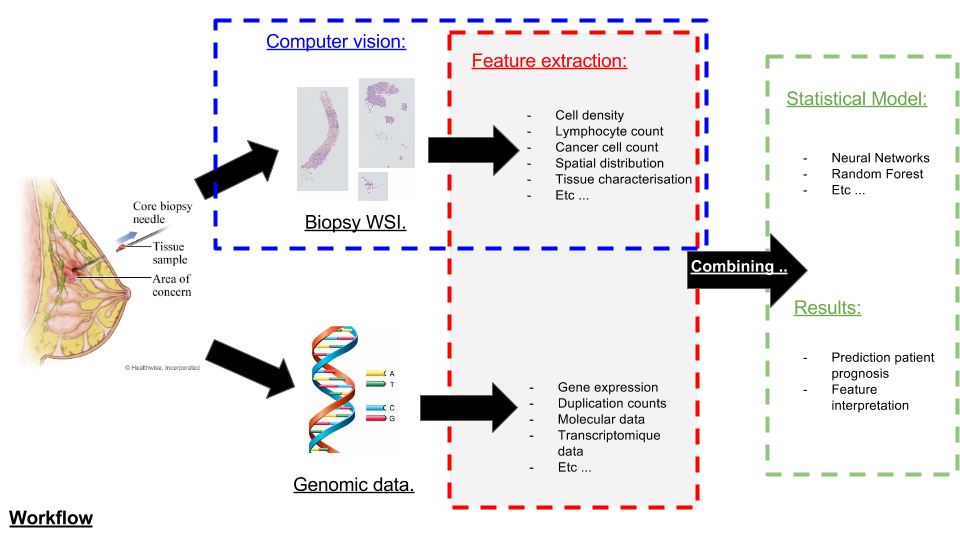
\includegraphics[width=\textwidth]{Workflow_overview.png}
\caption{Workflow}
\label{workflow1}
\end{figure*}

\begin{figure*}[!ht]
\centering
\begin{subfigure}{.3\textwidth}
  \centering
  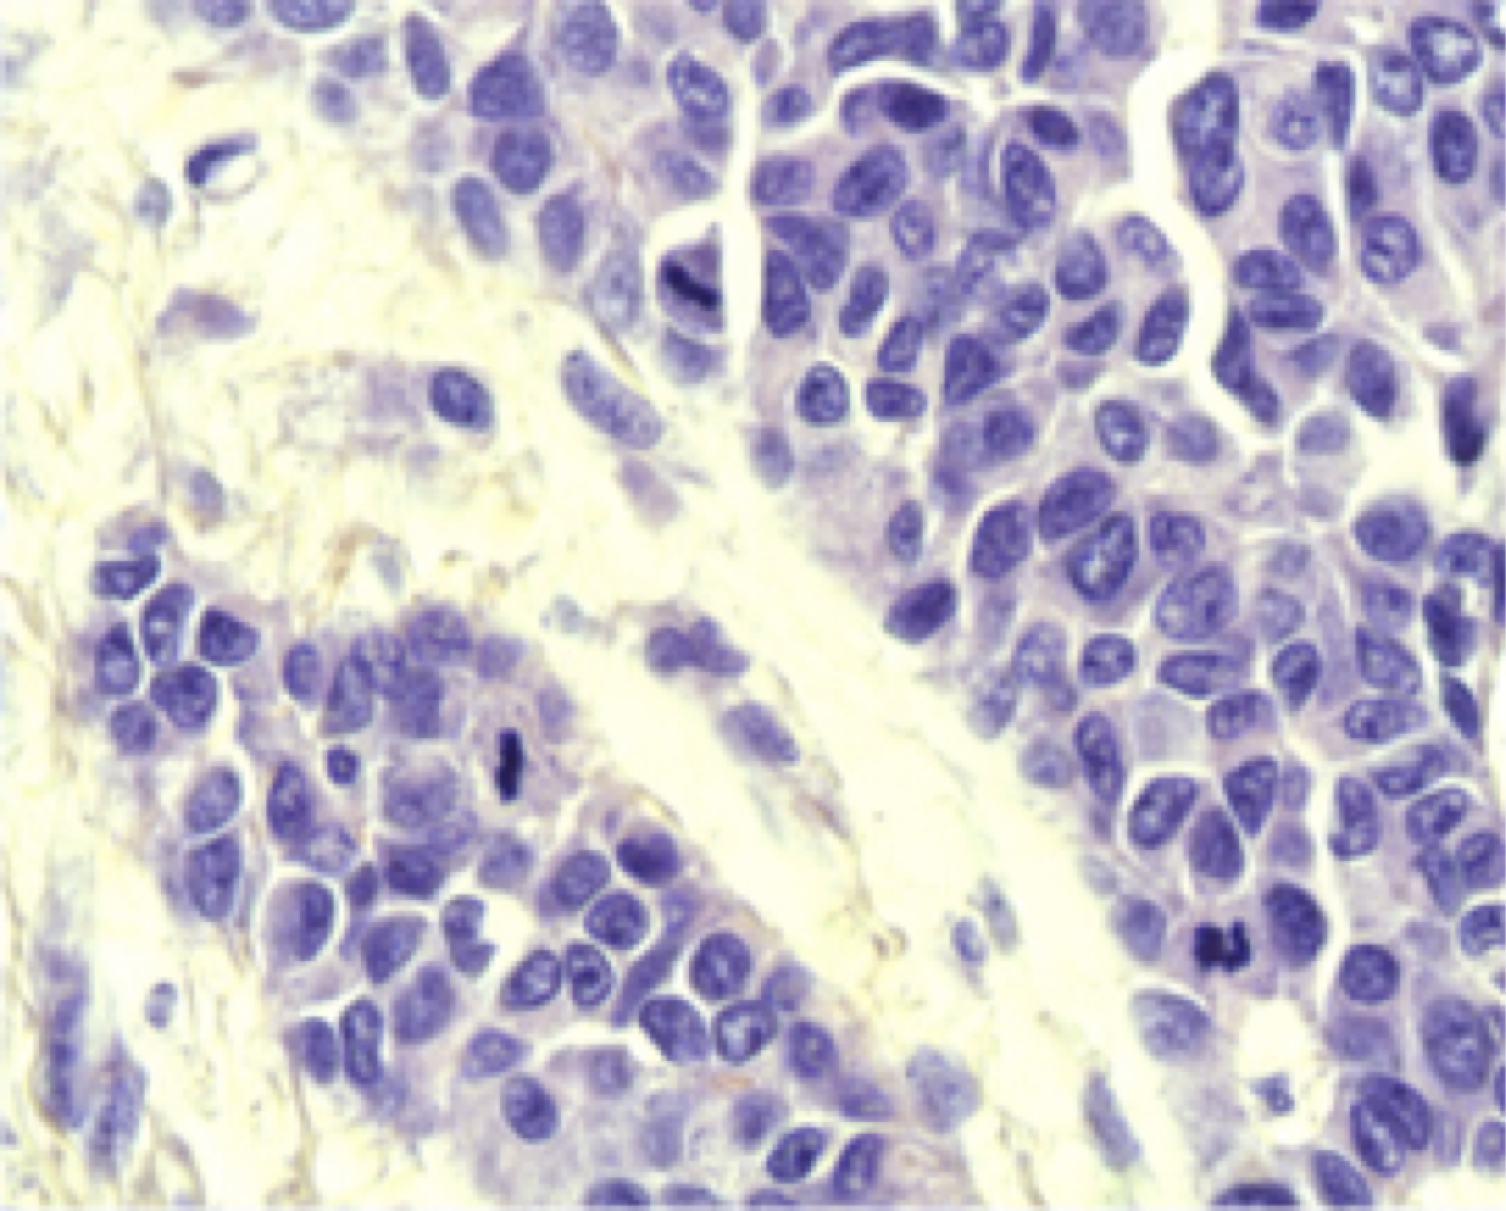
\includegraphics[height=4cm]{histo1.png}
  \caption{}
  \label{fig:sub1}
\end{subfigure}%
~
\begin{subfigure}{.3\textwidth}
  \centering
  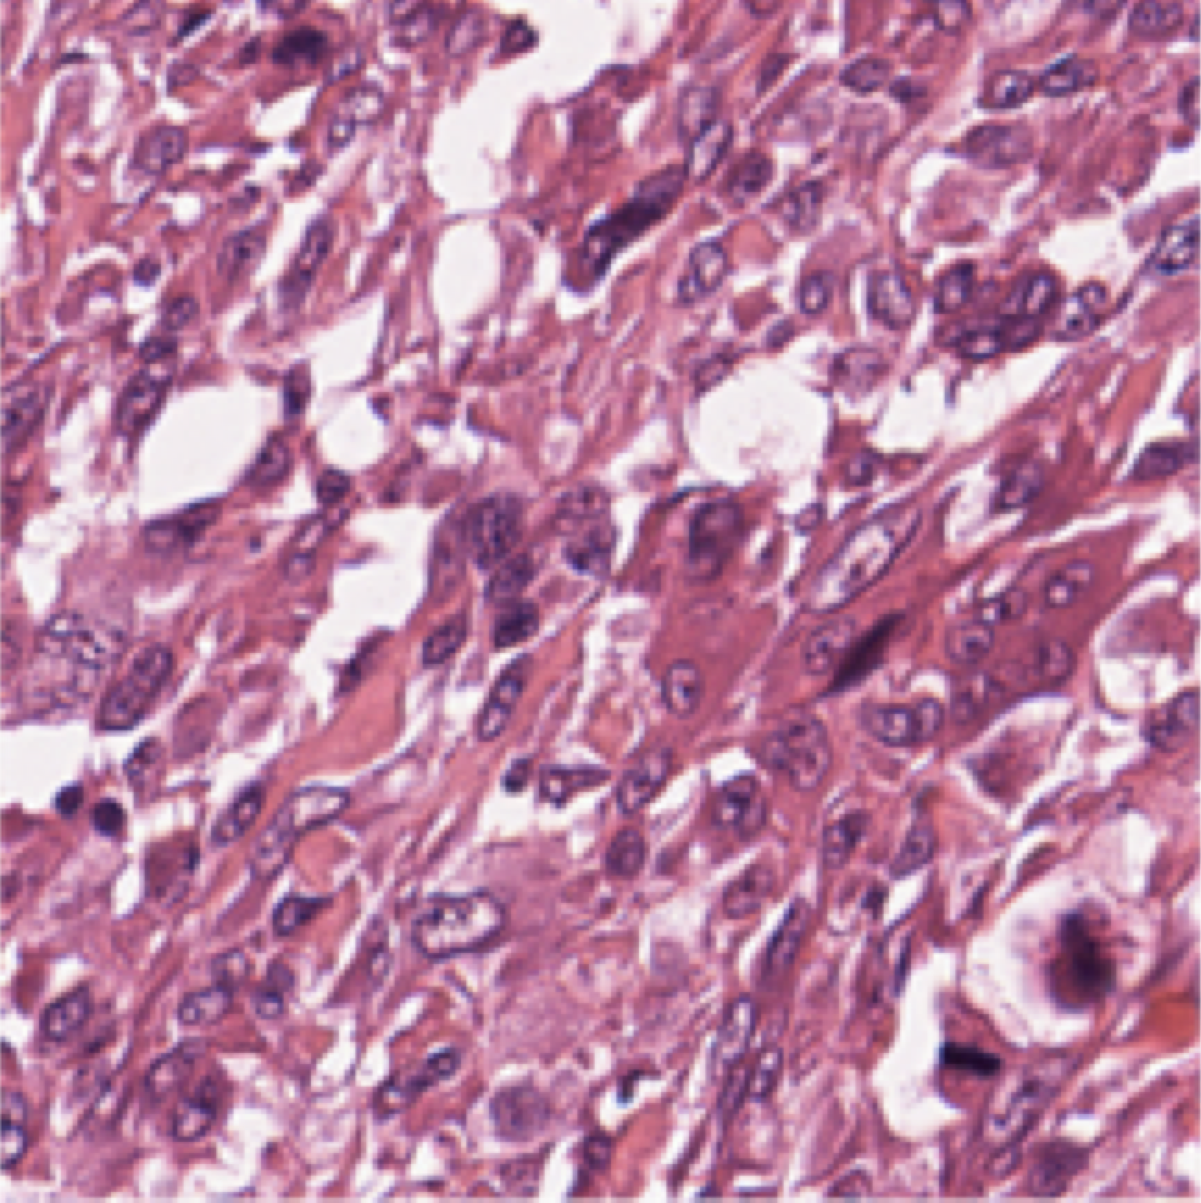
\includegraphics[height=4cm]{histo2.png}
  \caption{}
  \label{fig:sub2}
\end{subfigure}
~
\begin{subfigure}{.3\textwidth}
  \centering
  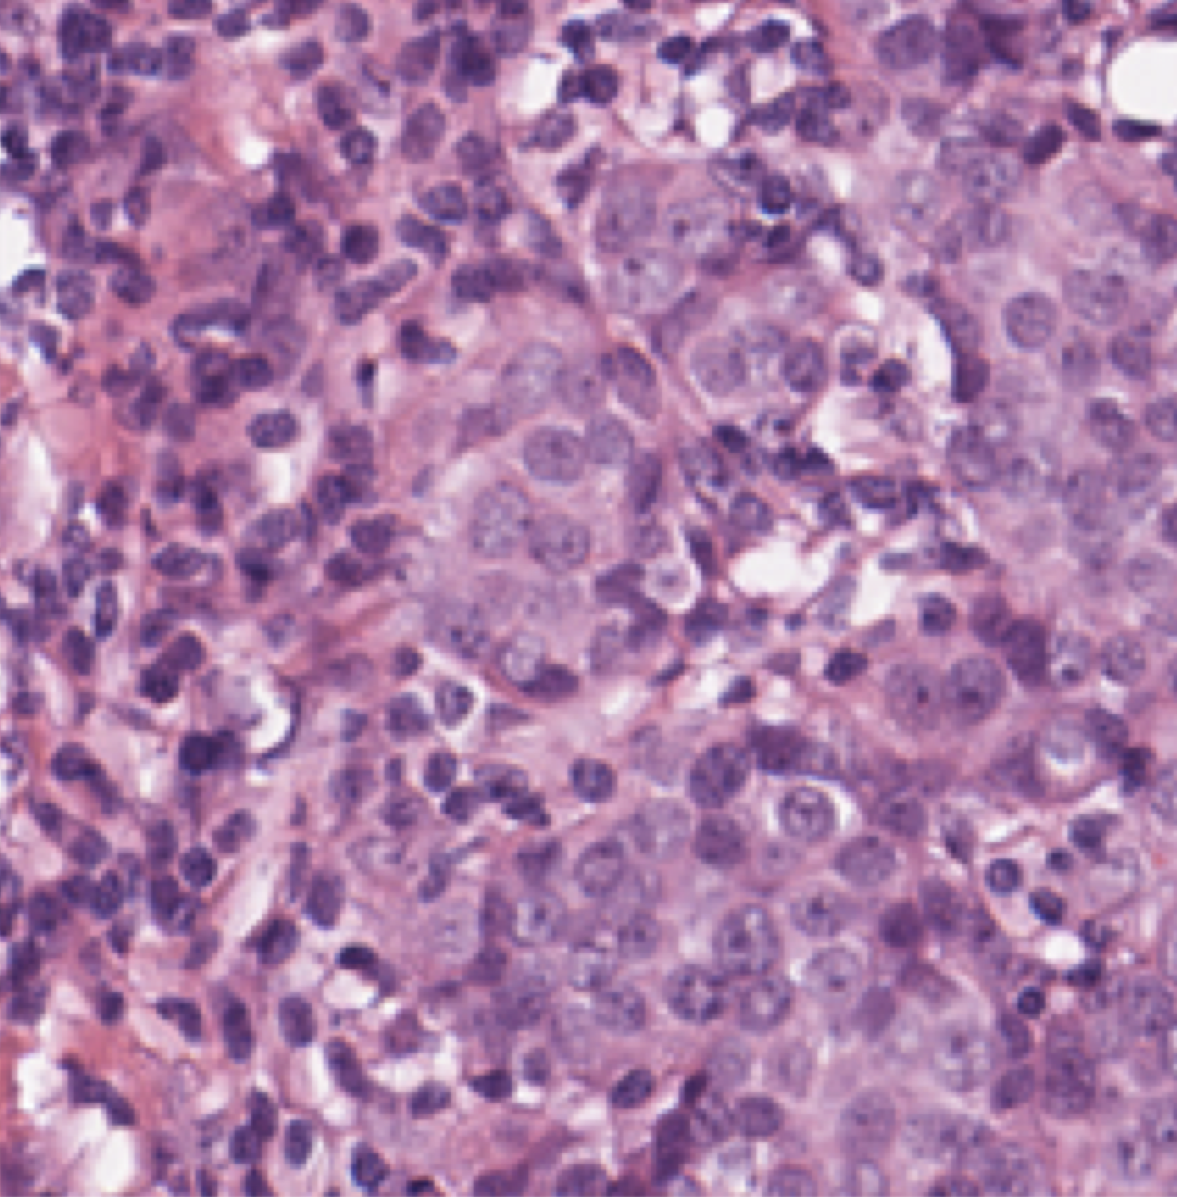
\includegraphics[height=4cm]{histo3.png}
  \caption{}
  \label{fig:sub3}
\end{subfigure}
\caption{Tissue sections with standard Haematoxylin and Eosin staining.}
\label{fig:example_histopath}
\end{figure*}



\end{document}